\section{Introduction}
\label{s:lab2-introduction}
Active enumeration is when a user programmatically gather informations on a system through
the use of a set of predefined commands. The most common set of informations that is
usually gathered through enumeration are DNS, IPs, ports, and services.

\begin{figure}[H]
  \centering
  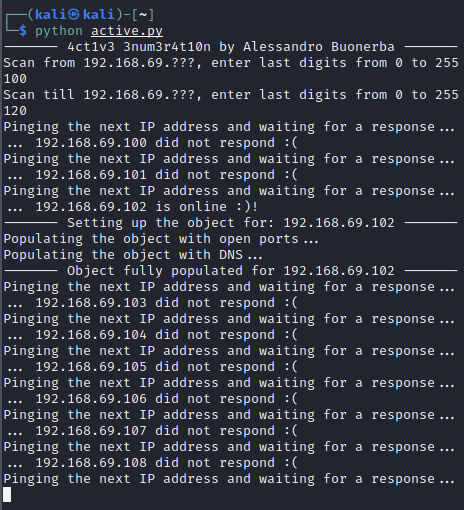
\includegraphics[width=0.5\textwidth]{figures/scrolling-text}
  \caption{scrolling-text}
  \label{f:scrolling-text}
\end{figure}

\begin{figure}[H]
  \centering
  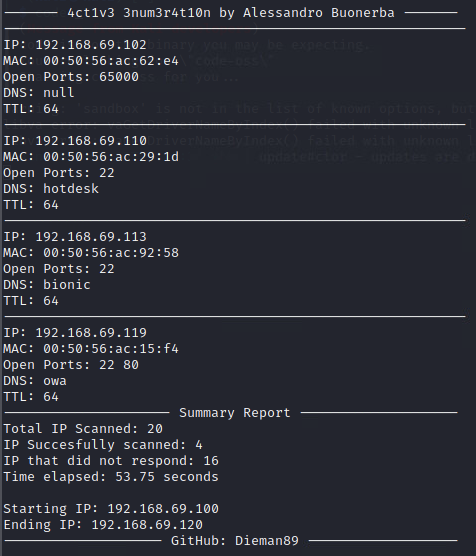
\includegraphics[width=0.5\textwidth]{figures/result-active-enum}
  \caption{result-active-enum}
  \label{f:result-active-enum}
\end{figure}

\begin{figure}[H]
  \centering
  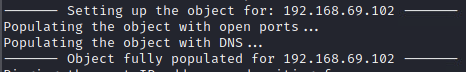
\includegraphics[width=0.7\textwidth]{figures/object-populating}
  \caption{object-populating}
  \label{f:object-populating}
\end{figure}

\section{Python Code}
\label{s:lab2-python-code}

\begin{figure}[H]
  \centering
  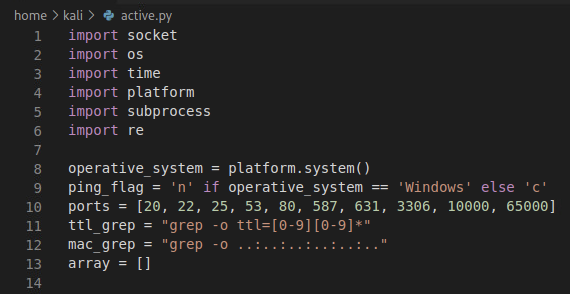
\includegraphics[width=0.7\textwidth]{figures/code/imports-declarations}
  \caption{imports-declarations}
  \label{f:imports-declarations}
\end{figure}

\begin{figure}[H]
  \centering
  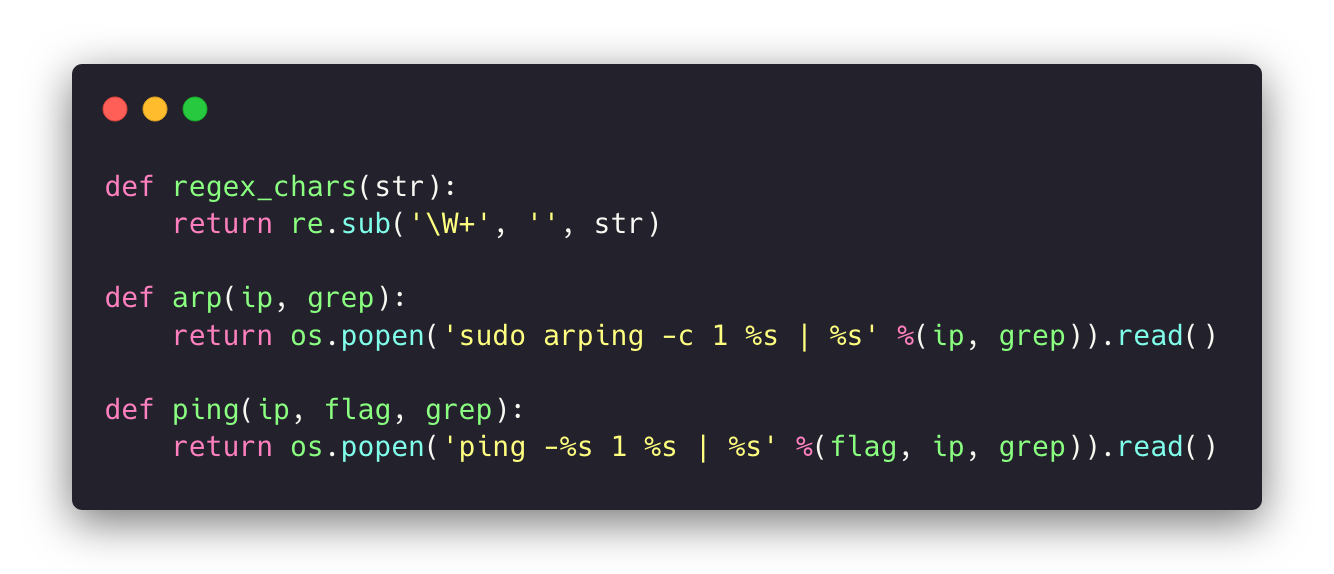
\includegraphics[width=0.7\textwidth]{figures/code/regex-arp-ping}
  \caption{regex-arp-ping}
  \label{f:regex-arp-ping}
\end{figure}

\begin{figure}[H]
  \centering
  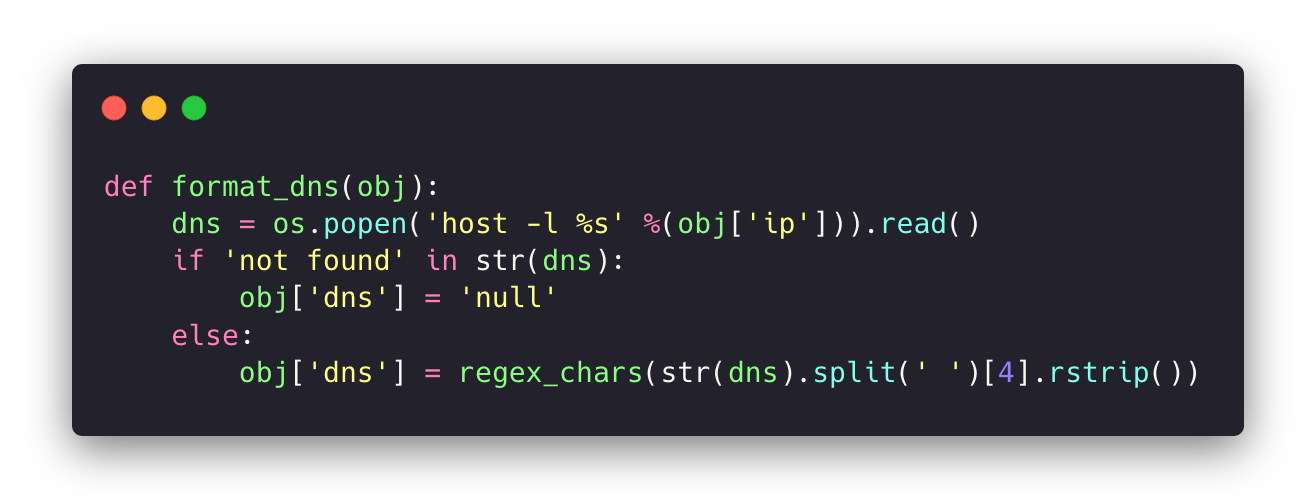
\includegraphics[width=0.7\textwidth]{figures/code/format-dns}
  \caption{format-dns}
  \label{f:format-dns}
\end{figure}

\begin{figure}[H]
  \centering
  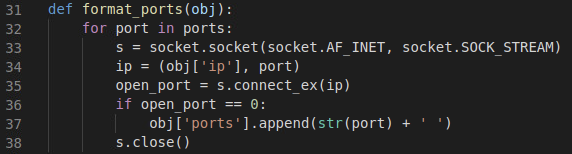
\includegraphics[width=0.7\textwidth]{figures/code/format-ports}
  \caption{format-ports}
  \label{f:format-ports}
\end{figure}

\begin{figure}[H]
  \centering
  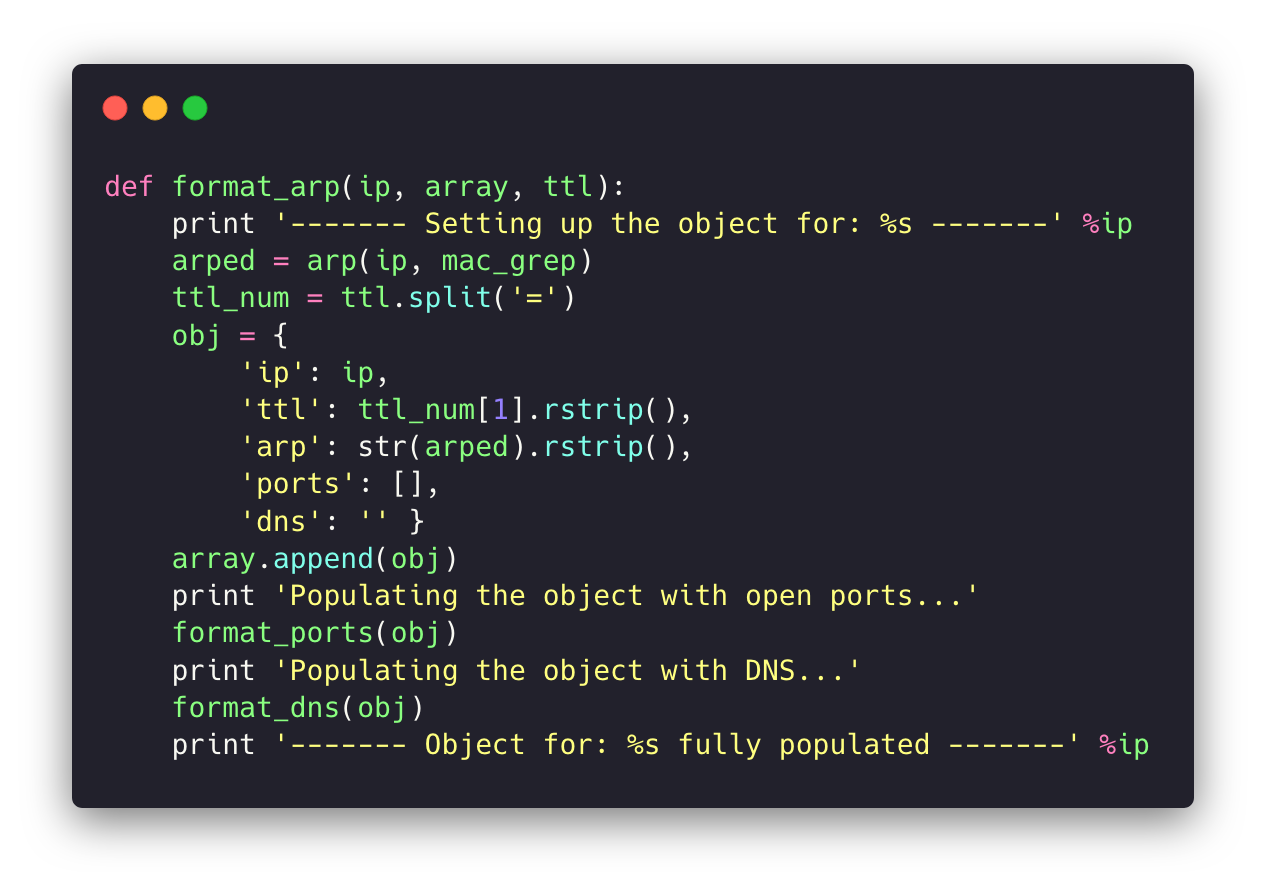
\includegraphics[width=0.7\textwidth]{figures/code/format-arp}
  \caption{format-arp}
  \label{f:format-arp}
\end{figure}

\begin{figure}[H]
  \centering
  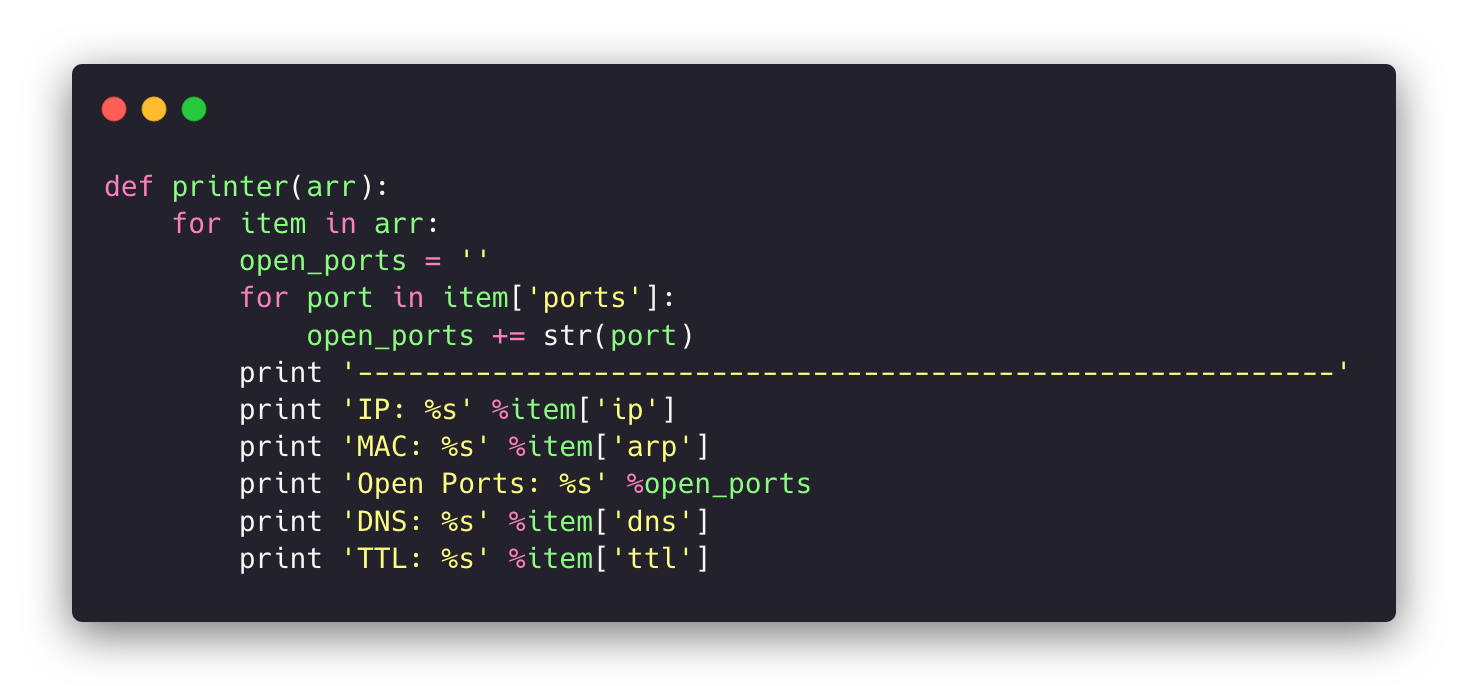
\includegraphics[width=0.7\textwidth]{figures/code/printer}
  \caption{printer}
  \label{f:printer}
\end{figure}

\begin{figure}[H]
  \centering
  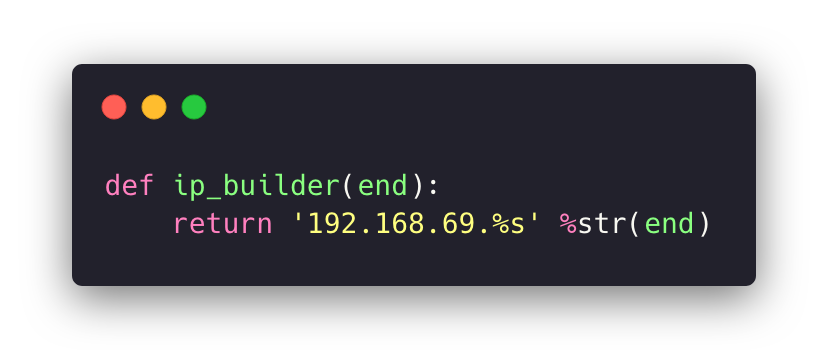
\includegraphics[width=0.7\textwidth]{figures/code/ip-builder}
  \caption{ip-builder}
  \label{f:ip-builder}
\end{figure}

\begin{figure}[H]
  \centering
  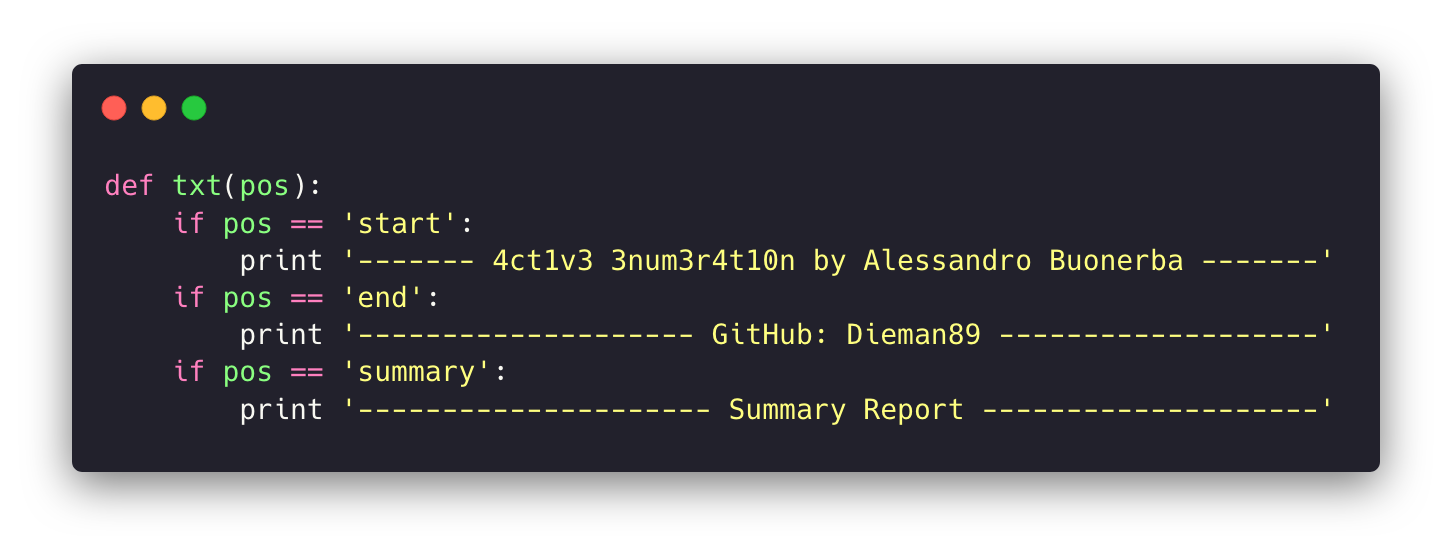
\includegraphics[width=0.7\textwidth]{figures/code/txt}
  \caption{txt}
  \label{f:txt}
\end{figure}

\begin{figure}[H]
  \centering
  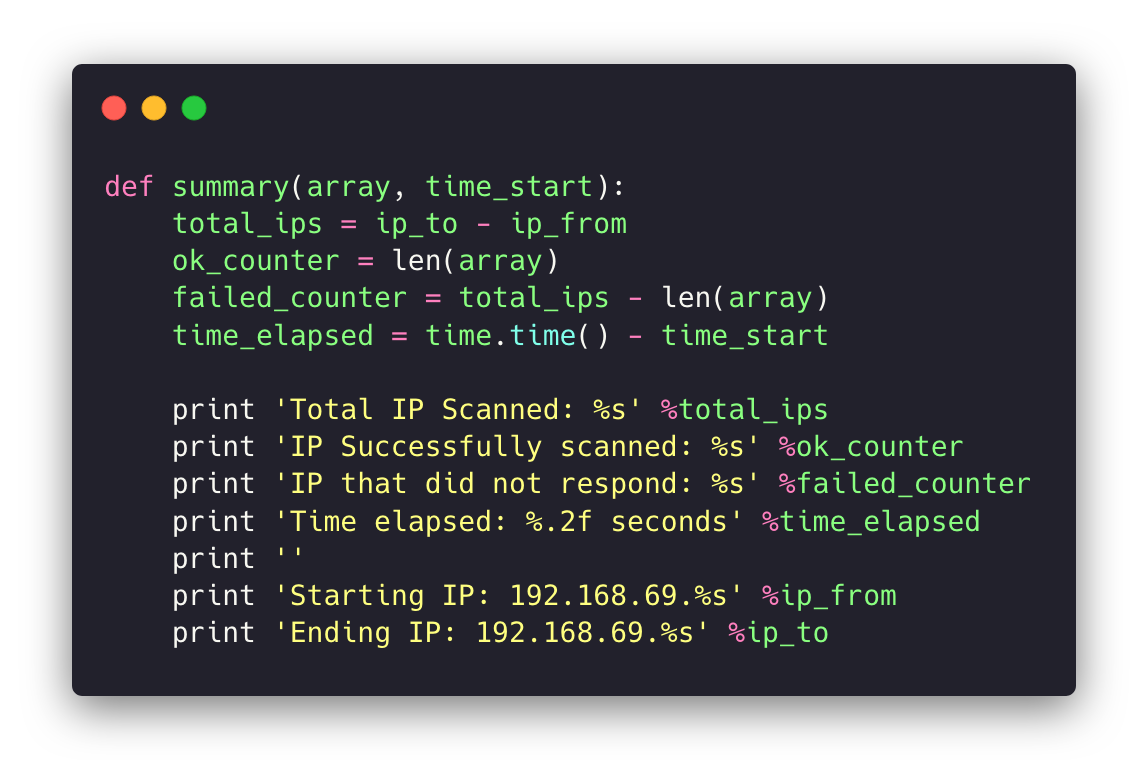
\includegraphics[width=0.7\textwidth]{figures/code/summary}
  \caption{summary}
  \label{f:summary}
\end{figure}

\begin{figure}[H]
  \centering
  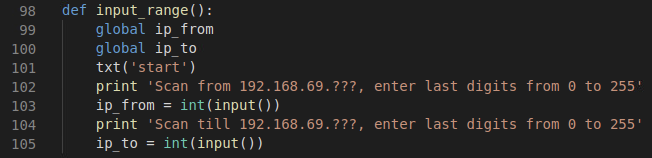
\includegraphics[width=0.7\textwidth]{figures/code/input-range}
  \caption{input-range}
  \label{f:input-range}
\end{figure}

\begin{figure}[H]
  \centering
  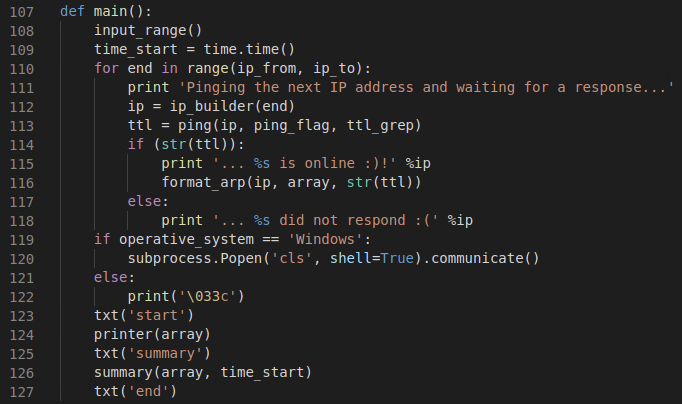
\includegraphics[width=0.7\textwidth]{figures/code/main}
  \caption{main}
  \label{f:main}
\end{figure}

\begin{figure}[H]
  \centering
  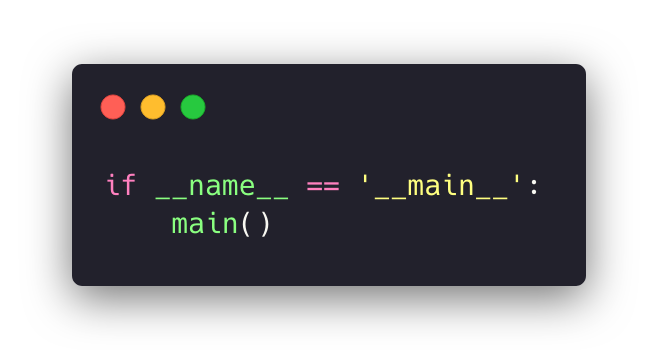
\includegraphics[width=0.7\textwidth]{figures/code/namemain}
  \caption{namemain}
  \label{f:namemain}
\end{figure}
